\documentclass{erdc}
\usepackage{lipsum,url}
\begin{document}

\frontmatter

%\laboratory{Cold Regions Research and\\ Engineering Laboratory}

\reportnum{ERDC/CRREL SR-05-78}

\program{Military Engineering Technology}

\title{Donec Felis
  Erat, Congue Non, Volutpat At, Tincidunt Tristique, Libero}

\subtitle{Nam feugiat lacus vel est, Version~1.0}

\date{March 2009\\Revised November 2010}

\author{A.U.~Thor \and C.O.R.~Respondent \and C.O.~Author}

\affiliation{Construction Engineering Research Laboratory\\
  U.S. Army Engineer Research and Development Center\\
  2902 Newmark Drive\\
  Champaign, IL 61826-9005}

\author{John~M.~Smith}

\affiliation{Coastal and Hydraulics Laboratory\\
  U.S. Army Engineer Research and Development Center\\
  3909 Halls Ferry Road\\
  Vicksburg, MS 39180-6199}

\coverart{nola}

\reporttype{Final Report}

% \distribution{Distribution authorized to U.S. Government Agencies
% only; Test and Evaluation; November 2005.  Other requests should be
% referred to U.S. Army Engineer Research and Development Center}

\additionalinfo{Supersedes ERDC/CREL AF-01-23}

\begin{abstract}
  \lipsum[12-13]
\end{abstract}

%\disclaimer{Some other disclaimer}

%\preparedfor{U.S. Army Engineer Research and Development Center\\
% 3909 Halls Ferry Road, Vicksburg, MS 39180-6199} 

\contractnum{Work Unit 33143}

\monitoredby{U.S. Army Engineer Research and Development Center\\
  3909 Halls Ferry Road, Vicksburg, MS 39180-6199}

%\preparedfor{}

\maketitle

\tableofcontents

\listoffiguresandtables

\chapter{Preface}
\lipsum[1-5]

\chapter{Unit Conversion Factors}

{\footnotesize\sffamily\centering
  \begin{longtable}{||l|l|l||}
    \hline\hline
    \bfseries Multiply & \bfseries By & \bfseries To Obtain\\
    \hline\hline
    \endhead
    \hline\hline
    \endfoot
    acres & 4,046.873 & square meters\\
    \hline
    acre-feet & 1,233.5 & cubic meters\\
    \hline
    angstroms & 0.1 & nanometers\\
    \hline
    atmosphere (standard) & 101.325 & kilopascals\\
    \hline
    bars & 100 & kilopascals\\
    \hline
    British thermal units (International Table) & 1,055.056 & joules\\
    \hline
    centipoises & 0.001 & pascal seconds\\
    \hline
    centistokes & 1.0E-06 & square meters per second\\
    \hline
    cubic feet & 0.02831685 & cubic meters\\
    \hline
    cubic inches & 1.6387064E-05 & cubic meters\\
    \hline
    cubic yards & 0.7645549 & cubic meters\\
    \hline
    degrees (angle) & 0.01745329 & radians\\
    \hline
    degrees Fahrenheit & (F-32)/1.8 & degrees Celsius\\
    \hline
    fathoms & 1.8288 & meters\\
    \hline
    feet & 0.3048 & meters\\
    \hline
    foot-pounds force & 1.355818 & joules\\
    \hline
    gallons (U.S. liquid) & 3.785412E-03 & cubic meters\\
    \hline
    hectares & 1.0E+04 & square meters\\
    \hline
    horsepower (550 foot-pounds force per second) & 745.6999 & watts\\
    \hline
    inches & 0.0254 & meters\\
    \hline
    inch-pounds (force) & 0.1129848 & newton meters\\
    \hline
    kilotons (nuclear equivalent of TNT) & 4.184 & terajoules\\
    \hline
    knots & 0.5144444 & meters per second\\
    \hline
    microinches & 0.0254 & micrometers\\
    \hline
    microns & 1.0E-06 & meters\\
    \hline
    miles (nautical) & 1,852 & meters\\
    \hline
    miles (U.S. statute) & 1,609.347 & meters\\
    \hline
    miles per hour & 0.44704 & meters per second\\
    \hline
    mils & 0.0254 & millimeters\\
    \hline
    ounces (mass) & 0.02834952 & kilograms\\
    \hline
    ounces (U.S. fluid) & 2.957353E-05 & cubic meters\\
    \hline
    pints (U.S. liquid) & 4.73176E-04 & cubic meters\\
    \hline
    pints (U.S. liquid) & 0.473176 & liters\\
    \hline
    pounds (force) & 4.448222 & newtons\\
    \hline
    pounds (force) per foot & 14.59390 & newtons per meter\\
    \hline
    pounds (force) per inch & 175.1268 & newtons per meter\\
    \hline
    pounds (force) per square foot & 47.88026 & pascals\\
    \hline
    pounds (force) per square inch & 6.894757 & kilopascals\\
    \hline
    pounds (mass) & 0.45359237 & kilograms\\
    \hline
    pounds (mass) per cubic foot & 16.01846 & kilograms per cubic meter\\
    \hline
    pounds (mass) per cubic inch & 2.757990E+04 & kilograms per cubic meter\\
    \hline
    pounds (mass) per square foot & 4.882428 & kilograms per square meter\\
    \hline
    pounds (mass) per square yard & 0.542492 & kilograms per square meter\\
    \hline
    quarts (U.S. liquid) & 9.463529E-04 & cubic meters\\
    \hline
    slugs & 14.59390 & kilograms\\
    \hline
    square feet & 0.09290304 & square meters\\
    \hline
    square inches & 6.4516E-04 & square meters\\
    \hline
    square miles & 2.589998E+06 & square meters\\
    \hline
    square yards & 0.8361274 & square meters\\
    \hline
    tons (force) & 8,896.443 & newtons\\
    \hline
    tons (force) per square foot & 95.76052 & kilopascals\\
    \hline
    tons (long) per cubic yard & 1,328.939 & kilograms per cubic meter\\
    \hline
    tons (nuclear equivalent of TNT) & 4.184E+09 & joules\\
    \hline
    tons (2,000 pounds, mass) & 907.1847 & kilograms\\
    \hline
    tons (2,000 pounds, mass) per square foot & 9,764.856 & kilograms per square meter\\
\hline
yards & 0.9144 & meters\\
\hline
\end{longtable}}

\mainmatter

\chapter{Duis ante felis, dignissim id, blandit in, suscipit vel,
  dolor}
\section{Duis ante felis: duis sagittis massa, dignissim id, blandit
  in, suscipit vel, dolor, nunc non magna}
\subsection{Nunc non magna: duis ante felis: duis sagittis massa,
  dignissim id, blandit in, vel dolor}
\lipsum[6]

\begin{equation}
  \label{eq:eq}
  2\times2=4
\end{equation}

\subsection{Duis sagittis massa}

\lipsum[7-9]

\section{Suscipit vel}

\lipsum[23]

\begin{enumerate}
\item Pellentesque laoreet velit nec justo.
\item Fusce consectetuer. Proin tellus est, luctus vitae,
  molestie a, mattis et, mauris. Donec tempor. Pellentesque habitant
  morbi tristique senectus et netus et malesuada fames ac turpis
  egestas. Duis ante felis, dignissim id, blandit in, suscipit vel,
  dolor. Pellentesque tincidunt cursus felis.
\item Proin rhoncus semper
  nulla. Ut et est. Vivamus ipsum erat, gravida in, venenatis ac,
  fringilla in, quam. Nunc ac augue. Fusce pede erat, ultrices non,
  consequat et, semper sit amet, urna.
\end{enumerate}

\lipsum[17-18]

\begin{table}
  \centering
  \caption{Yearly Dividens}
  \label{tab:dividends}
  \footnotesize\sffamily
  \begin{tabular}{||l|D{.}{.}{2.2}||}
    \hline\hline
    \textbf{Year}  &  \multicolumn{1}{|c||}{\textbf{Dividends, \%}}\\
    \hline\hline
    $1880$  & 2.50  \\
    \hline
    $1881$  & 12.1  \\
    \hline
    $1882$  & 2.6  \\
    \hline\hline
  \end{tabular}
\end{table}

\subsection{Sagittis massa}

\lipsum[24]

\begin{figure}
  \centering
  \fbox{
\includegraphics[width=2in]{red_corps_castle2}}
  \caption{Castle}
  \label{fig:castle}
\end{figure}

\lipsum[9]

\chapter{Duis sagittis massa in tellus}

\lipsum[11]

\begin{equation}
  \label{eq:B}
  \int P\,dx =1
\end{equation}

\begin{itemize}
\item Fusce adipiscing justo nec ante. Nullam in enim.
  Pellentesque felis orci, sagittis ac, malesuada et, facilisis in,
  ligula. Nunc non magna sit amet mi aliquam dictum. In mi.
\item Curabitur
  sollicitudin justo sed quam. Aenean imperdiet. Vestibulum ante ipsum
  primis in faucibus orci luctus et ultrices posuere cubilia Curae;
  Donec lacinia nonummy lectus. Proin vel urna. Fusce sit amet orci ac
  magna iaculis pharetra. Duis sagittis massa in tellus.
\end{itemize}

\section{Fusce consectetuer}

\lipsum[10]

\begin{figure}
  \centering
  \fbox{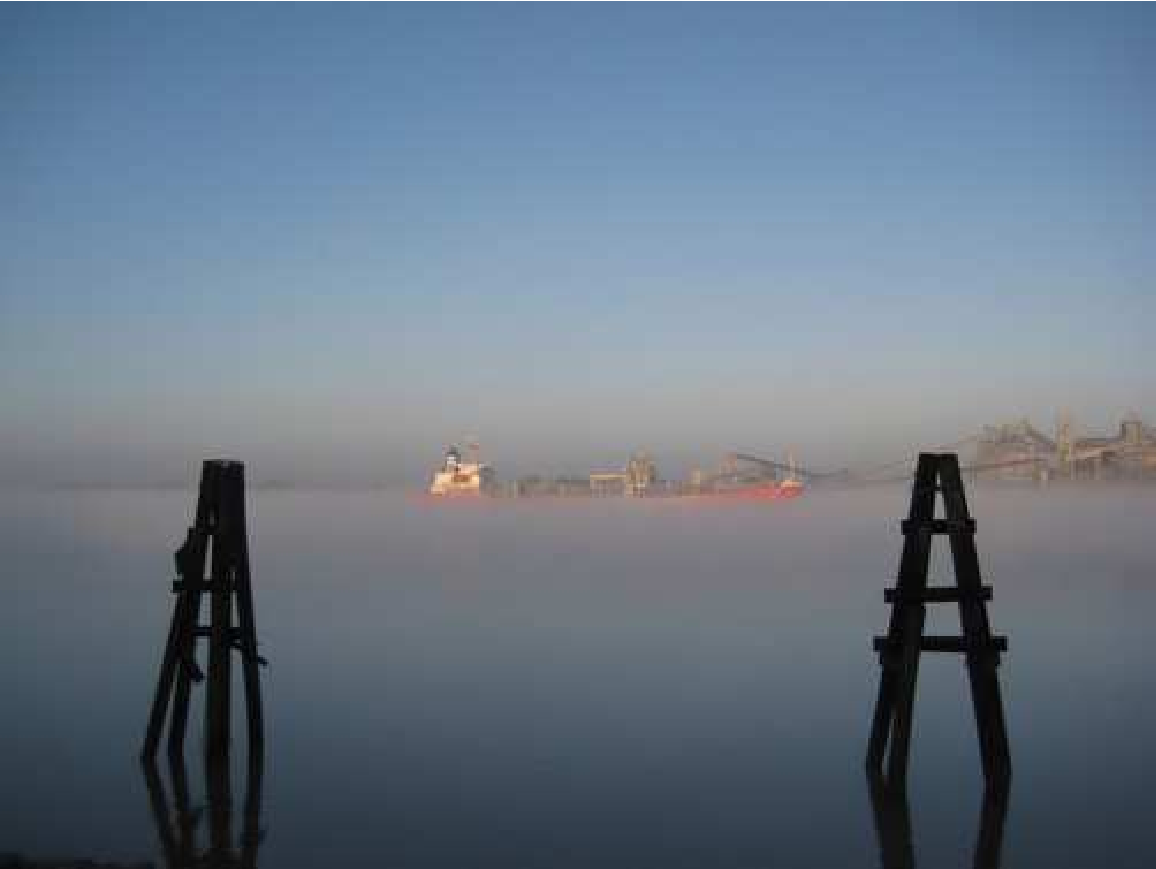
\includegraphics[width=4in]{nola}}
  \caption{A Picture From US Army Corps Of Engineers Site}
  \label{fig:nola}
\end{figure}

\section{Aenean imperdiet}

\lipsum[11]

\nocite{*}

\bibliographystyle{unsrt}
\bibliography{erdc}

\appendix

\chapter{Aenean imperdiet}

\lipsum[12-16]

\begin{equation}
  \label{eq:C}
  \frac{\partial H}{\partial x} = -X
\end{equation}

\begin{figure}
  \centering
  \fbox{
\includegraphics[width=2in]{red_corps_castle2}}
  \caption{Another Castle, Now In Appendix}
  \label{fig:castle1}
\end{figure}

\lipsum[26]
\lipsum[32]

\begin{equation}
  \label{eq:D}
  e^{i\pi} + 1 = 0
\end{equation}

\begin{table}
  \centering
  \caption{Dam on Table Rock Lake}
  \label{tab:Dam}
  \footnotesize\sffamily
  \begin{tabular}{|l|r|}
    \hline
    Length of dam, feet &6,423\\
    \hline
    Concrete section, feet &1,602\\
    \hline
    Earth embankment feet &4,821\\
    \hline
    Maximum height of dam above streambed, feet &252\\
    \hline
    Concrete in dam, cubic yards &1,230,000\\
    \hline
    Earth in embankment, cubic yards &3,320,000\\
    \hline
    Length of spillway, gross feet &531\\
    \hline
    Spillway crest gates (10), size in feet &45x37\\
    \hline
    Outlet conduits (4), size in feet &4x9\\
    \hline
    Elevations, feet above mean sea level & \\
    \hspace{20pt}Top of dam & 947\\
    \hspace{20pt}Spillway crest & 896\\
    \hline
  \end{tabular}
\end{table}

\lipsum[27]

\chapter{Pellentesque habitant
  morbi tristique senectus et netus et malesuada fames ac turpis
  egestas}

\lipsum[16-22]
\begin{equation}
  \label{eq:U}
  S = -kT\ln\Xi
\end{equation}
See equation~(\ref{eq:C}) and equation~\eqref{eq:D}.

\begin{figure}
  \centering
  \fbox{
\includegraphics[width=2in]{red_corps_castle2}}
  \caption{Yet Another Castle In Appendix}
  \label{fig:castle2}
\end{figure}


\end{document}
